
\documentclass[mathserif]{beamer}

\mode<presentation>
{
  %\usetheme{Warsaw}
  %\usetheme{Adelaide}
  %\usetheme{default}
  %\setbeamercovered{transparent}
  \setbeamertemplate{navigation symbols}{}
}

% adapt beamer style
%\setbeamercolor{block title}{fg=titleblue}
\definecolor{titleblue}{rgb}{0.29,0.41,0.58}
\definecolor{myred}{rgb}{0.81,0.23,0.16}
%\definecolor{mygreen}{rgb}{0.36,0.54,0.33}
\definecolor{mygreen}{rgb}{0.21,0.40,0.12}

\usepackage[english]{babel}
%\usepackage[latin1]{inputenc} % on unix
\usepackage[applemac]{inputenc} % on mac
\usepackage[T1]{fontenc}

%\usepackage[usenames,dvipsnames]{color}
%\usepackage[dvips]{color}
\xdefinecolor{mylightgrey}{gray}{0.7}

\usepackage{amsmath}
%\usepackage{amssymb}
%\usepackage{amsfonts}
\usepackage{rotating}

%\usepackage{concmath}
\usepackage{times}

\usepackage{prompt}

% a few new commands
\newcommand{\C}{\mathcal{C}}
\newcommand{\E}{\mathsf{E}}
\DeclareMathOperator*{\argmax}{arg\,max}
\newcommand{\supp}{\mathcal{S}}
\newcommand{\Xset}{\mathcal{X}}
\newcommand{\BEP}{{\mathsf{BEP}}}
\newcommand{\BSC}{{\mathsf{BSC}}}
\newcommand{\BEC}{{\mathsf{BEC}}}

\definecolor{myblue}{rgb}{0.05,0.05,0.7}
\newcommand{\textbfblue}[1]{\textcolor{myblue}{\textbf{#1}}}
\definecolor{lightgray}{gray}{0.95}

\title{Extremes of Gallager's error exponents}

\author{%
Ingmar Land \\[1ex]
\footnotesize
Institute for Telecommunications Research \\
University of South Australia}

\date{AusCTW Wellington \\ 31 Jan 2012} 

%-----------------------------------------------------------

\begin{document}

\begin{frame}
  \titlepage
\end{frame}

\silence

\begin{frame}
  \frametitle{} 
  
  \centering
  \vspace{2ex}
  \begin{turn}{1}
  %\begin{turn}{0}
  \hspace{4ex}
  \begin{minipage}{0.8\textwidth}
  \begin{block}{Outline}
    \begin{enumerate}
    \item Binary-input symmetric memoryless channels
    %\item Extremes of bit error probability
    \item Gallager exponents
    \item Extremes of Gallager exponents
    %\item proofs
    \end{enumerate}
  \end{block}
  \end{minipage}
  \end{turn}
  
  \vspace{5ex}
  \begin{turn}{-1}
  %\begin{turn}{0}
  \hspace{2ex}
  \begin{minipage}{0.8\textwidth}
  \begin{block}{}
    Joint work with \\
  Albert Guill\'en i F\`abregas and Alfonso Martinez \\
  Universitat Pompeu Fabra, Spain
  \end{block}
  \end{minipage}
  \end{turn}
\end{frame} 

\attention

\begin{frame}{}  
  %\vspace{1ex}
  \begin{block}{Theorem (Extremes of Gallager exponents)}
  \vspace{1ex}
  %\textbf{Theorem}: \; 
  For any BISMC with capacity $C$,
  \begin{equation*}
    E_r^\BSC(R;C) \;\le\; E_r(R;C) \;\le\; E_r^\BEC(R;C) ,
  \end{equation*}
	and the bounds are achieved by the BSC and the BEC.
  %\vspace{1ex}
%  \begin{center}
%    \includegraphics[scale=0.45]{error_exponents_bec_bsc_bpsk_c_Albert}
%	\end{center}
	\end{block}
\end{frame}

\surprise

\begin{frame}
  \centering
  \vspace{-2ex}
  \begin{turn}{8}
  %\begin{turn}{0}
  \hspace{-6ex}
  \begin{minipage}{0.8\textwidth}
  \begin{block}{Summary}  
    \vspace{1ex}  
    For any BISMC with capacity $C$, \\[1ex]
    $\BSC \le \text{Gallager exponent}   \le \BEC$.
%    \begin{itemize}
%      \item $\BSC \le \text{bit error probability}   \le \BEC$
%      \item $\BSC \le \text{Gallager exponent}     \,\le \BEC$
%    \end{itemize}
  \end{block}
  \end{minipage}
  \end{turn}

  \vspace{2ex}
  \hspace{18ex}
  \begin{turn}{-2}
  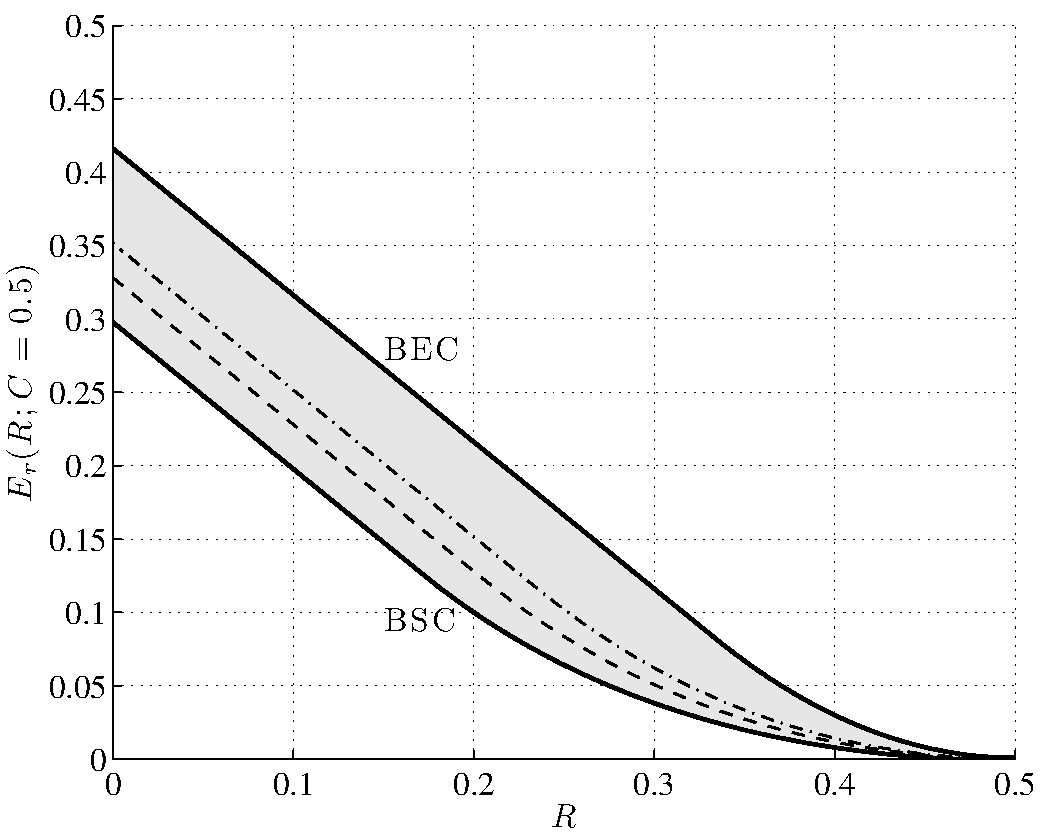
\includegraphics[scale=0.35]{examplefig.pdf}
  \end{turn}
\end{frame} 

\applause

\end{document}
